\scanpage{61}
$\handwritten{\mathcal{M}}$ en termes de la f\unsure{\deleted{ma}am|\deleted{am}ma}ille des $A_i$ \deleted{et des entiers $d_i=\operatorname{rang}E_i$} comme suit\deleted{e}. On considère d'abord la catégories sous-additive \deleted{engendrée} ayant comme objets les éléments $\handwritten{\underline{\gamma}}$ de $\underline{N}^{(I)}$, ($\handwritten{\underline{\gamma}}=(\handwritten{\gamma}_i)_{i\handwritten{\in}I}$ étant interprété comme $\handwritten{\bigotimes}E_i^{\handwritten{\gamma}_i}$), \deleted{ou} avec $\operatorname{Hom}(\handwritten{\underline{\gamma}},\handwritten{\underline{\gamma}'})=0$ si $\handwritten{\underline{\gamma}\ne\underline{\gamma}'}$ et $=\bigotimes_{\handwritten{i}} A_i^{\otimes\handwritten{\gamma_i}}$ si $\handwritten{\underline{\gamma}=\underline{\gamma}'}$, la composition des morphismes évidentes. On définit de façon évidente le foncteur $\otimes$ (addition de $\underline{N}^{(I)}$ sur les objets, produit tensoriel sur les homomorphismes) et ses constra\unsure{\deleted{ntn}int|\deleted{int}ntn}es,\margin{\handwritten{\unsure{attention|attent°} à\\contrainte de\\commutativité}} de façon que l'on trouve une sous-$\otimes$-catégorie. Son enveloppe Karoubienne est une\inserted{$\otimes$-\begin{tikzpicture}[x=1cm,y=1cm,baseline=-.1cm]\draw[thin] (0,.2).. controls (-.3,-.1) and (-.85,.1)..(-1.05,-.16).. controls (-1.2,-.3) and (-1.25,-.4)..(-1.15,-.55);\end{tikzpicture}}catégorie abélienne, qui s'identifie à la sous-catégorie pleine de $\handwritten{\mathcal{M}}$ formée des éléments dont les composantes homogènes non nulles sont à degrés $\handwritten{\in}\underline{N}^{(I)}$,\inserted{et a un foncteur fibre sur \deleted{$\unsure{k|K}$}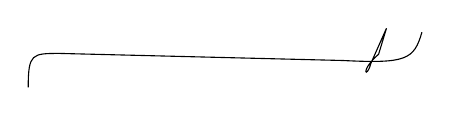
\begin{tikzpicture}[x=1cm,y=1cm,baseline=-.1cm]\draw[thin] (0,.3).. controls (-.1,-.05) and (-.2,-.1)..(-1,-.06)--(-4.6,.03).. controls (-4.95,.03) and (-5,.03)..(-5,-.4);\draw[thin] (-.45,.35)--(-.55,.02).. controls (-.8,-.2) and (-.7,-.3)..(-.65,-.1)--(-.45,.35);\end{tikzpicture}}\margin{$\overset{\handwritten{-}}{k}$.\makebox[0pt][l]{
\begin{tikzpicture}[x=1cm,y=1cm,baseline=0pt]\draw[thin] (-.22,.12) ellipse (.4 and .3);\draw[thin] (-.63,.28)--(-.71,-.1).. controls (-.88,-.31) and (-.81,-.34)..(-.76,-.2)--(-.63,.28);\end{tikzpicture}}} D'autre part, pour tout $i$, si $A_i$ est de \deleted{degré}\inserted{rang} $d_i^2$ (donc $E_i$ de rang $d_i$), soit $L_i=\det E_i={\handwritten{\unsure{A|\bigwedge}_{\unsure{k|t|2}}}}^{d_i}\handwritten{E_i}$ (où $E_i$ désigne l'objet de la catégorie construite correspondant \deleted{à l'} $i$.ème élément de la base canonique de $\underline{Z}^{(I)}$, soit $\unsure{1|l}_i$ ...), c'est un objet préinversible ($\inserted{\handwritten{X\to\begin{tikzpicture}[x=1cm,y=1cm,baseline=-.1cm]\draw[thin] (0,.2).. controls (-.3,-.1) and (-.85,.1)..(-1.05,-.16).. controls (-1.2,-.3) and (-1.25,-.4)..(-1.15,-.55);\end{tikzpicture}}}\deleted{\unsure{\otimes}}L_i\otimes\handwritten{X}$ est pleinement fidèle) et en inversant les $L_i$, on trouve (à \deleted{équ}équivalence près\deleted{\unsure{)|t|?}} respectant tout) la catégorie $\handwritten{\mathcal{M}}$.

Quand $\handwritten{\Gamma}$ n'est pas libre, on trouve une construction analogue en termes d'un système de générateurs\inserted{convenable\begin{tikzpicture}[x=1cm,y=1cm,baseline=-.1cm]\draw[thin] (0,.2).. controls (-.3,-.1) and (-.85,.1)..(-1.05,-.16).. controls (-1.2,-.3) and (-1.25,-.4)..(-1.15,-.55);\end{tikzpicture}} $(\handwritten{\gamma}_i)_{i\handwritten{\in}I}$, mais en``ren\unsure{\deleted{e}d|\deleted{a}d|\deleted{d}e|\deleted{d}a}ant \deleted{de plus} égaux à 1$^{\unsure{\deleted{I}|x|\deleted{x}|?}}$'' de plus certains éléments.\margin{A explici-\\ter !} Ces constructions sont bien adaptées pour décrire les $\otimes$-foncteurs de $\handwritten{\mathcal{M}}$ dans une \deleted{$\otimes$-}catégorie tannakienne, et pour décrire le changement de base.( Pour cette dernière raison notamment, il aurait été maladroit dans le cas général de prendre les $M_i$ simples ....). Attention, dans la description des $\otimes$-foncteurs en question, de tenir compte des c\unsure{\deleted{l}o|\deleted{o}l|\deleted{d}o}ntraintes, notamment de celle d\deleted{\unsure{'|i|?}}e commutativité; il semble qu'il doive revenir au même d'exiger que le rang est conservé ...
% archive sheet number: 60
